\documentclass{beamer}
\usepackage{multirow}
\usepackage{biblatex}
\usepackage[T1]{fontenc}
\usepackage{amsmath}
\usepackage{MnSymbol}
\usetheme{Madrid}
\title{Contagion Effect Estimate Through the Lens of Different Statistical Methods}
\author{Brisilda Ndreka\\
Department of Statistic\\
University of Connecticut
} 
\date{ December 5, 2022}

\begin{document}
\maketitle 
%=================================================
\begin{frame}
\frametitle{Outline}
\begin{itemize}
   \item  Influence model (behaviour) using dynamic linear model. 
     \vspace{10pt}
    \item Why is estimating contagion effect in social science considered a challenged  process?
    \vspace{10pt}
    \item Alternative methods which help to achieve a better estimation of the true contagion effects
    \vspace{10pt}
    \item  Defining the estimation method that has the  best performance
\end{itemize}
\end{frame}
%=================================================
\begin{frame}
\frametitle{Background}
\begin{itemize}
    \item Contagion effect also referred as social influence effect or peer effect, is the tendency of a person or group of individuals has to follow the behaviour of some reference group that they participate.
    \vspace{10pt}
    \item The dynamic liner model used to estimate social influence effect is referred to as behaviour model(Xu, 2018; Friedkin \& Johnsen, 1990)
  \begin{figure}[h!]
  \centering
  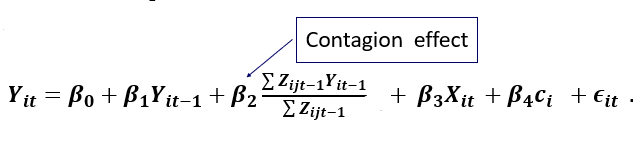
\includegraphics[width=.8\linewidth]{mod.png} 
\end{figure}
 $Y$ is the behavior outcome of interest, $X$ covariates that may affect behavioral outcome $Y$, $Z$ is network, $c$ is the time-invariant unobserved trait.  
\end{itemize}
\end{frame}
%=================================================
\begin{frame}
\frametitle{Why it is Difficult to Identifying Social Influence Effect (Contagion Effect)? }
\begin{itemize}
\item Consider the example: In daily life, friends in social networks exhibit similar personality  and behaviors. Why doe this phenomena happen? \\
Answering this questions can result in two in two direction thinking:
\vspace{10 pt}
\begin{itemize}
\item Social influence effect: Individuals can influence their friends behaviour, transform their friends characteristics to be similar to theirs. 
\vspace{10pt}
\item Homophily: In which people with similar characteristics or behaviors are more likely to be friends. 
\end{itemize}
\vspace{10 pt}
\item Consequently, homophily has been identified as a major confounding factor to estimate the influence in social network effect. 

\end{itemize}
\end{frame}
%=================================================
\begin{frame}
\frametitle{This Challenge can be Treated  as  a Function of an Omitted Variable Bias }
\begin{itemize}
\item{Separating homophily from  social influence is
a challenging process, particularly when  influence effect  is confounded with latent homophily caused by unobserved trait.}
\vspace{10pt}
\begin{itemize}
    \item If an unobserved variable affects behavioral model and selection process this cause estimation problems of the social influence effect (Xu, 2018; Shalizi \& Thomas 2011). Alcohol behaviour among teenager example.
    \begin{figure}[h!]
  \centering
  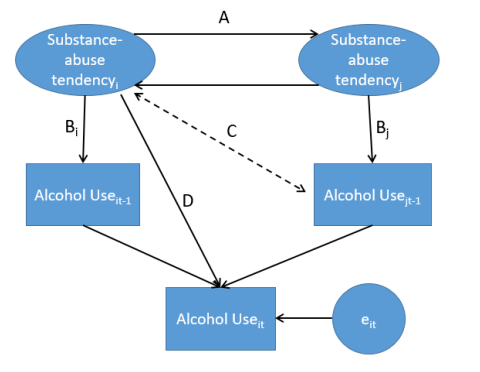
\includegraphics[width=.4\linewidth]{rx.png}
  \caption{Omitted variable bias/  (Xu, 2021)}
  \label{fig:fig1}
\end{figure}
\end{itemize}
\end{itemize}
\end{frame}
%=================================================
\begin{frame}
\frametitle{Estimation methods used to estimate latent variable :}
\begin{itemize}
\item Considering existence of biases of the contagion effects if omitted variables in the influence/selection process exist, four estimation methods are applied: 
\begin{itemize}
\begin{enumerate}
 \item Latent space  method (Xu, 2018).
\vspace{10pt}
\item SDNE: Structural Deep Network Embedding (Wang et al, 2016).
\vspace {10pt}
\item Node2Vec
\vspace {10pt}
\item Latent Factor Model
\end{enumerate}
\end{itemize}
\vspace {10pt}
\item Furthermore, fixed  effect estimator are used  as baseline comparisons. The objective of the study is to determine the method that has the best performance and help to reduce bias of estimating peer effect.
\end{itemize}
\end{frame}
%================================================
\begin{frame}
\frametitle{ I: Latent Space Adjusted Approach}
\begin{itemize}

\item Assume the existence of an unobserved trait that co-determines influence and selection process.
\vspace{10pt}
\item The information of unobserved trait from the selection proces as an estimator of the latent variable in the influence model.
\vspace{10}
\item  Estimation of $c$ is completed  using  "latent social positing" form the Latent space  models (Hoff, 2002), using ergmm package in R-software.
 \vspace{10pt}
  \item  By including the latent positions as additional covariates in the behavioral model it
will reduce the bias in the estimation of social influence effects.

\end{itemize}
\end{frame}
%================================================
\begin{frame}
\frametitle{ II: SDNE }
\begin{itemize}
\item  SDNE is machine learning algorithm  with the goal of turning a graph into a computationally  absorbable format. 
\vspace{10pt}
\item  Network embedding intend to capture and carry out the network structure of a network structure using low-dimensional representations of vertexes in networks. 
\vspace{10pt}
  \item   It is  a method that is
able to effectively capture the highly non-linear network structure.
\end{itemize}


\end{frame}
%=================================================

\begin{frame}
\frametitle{ Nde2vec}
\begin{itemize}
\item  Node2vec is a random walk based method, which  use a walk approach to generate (sample) network neighborhoods for nodes. 
\vspace{10 pt}
\item Algorithm computes a vector representation of a node based on random walks in the graph.
\vspace{10 pt}
\item  Two parameters control the probability of moving in the graph.
\begin{itemize}
\item return hyperparameter, p 
\item inout hyperparameter, q 
\begin{figure}[h!]
  \centering
  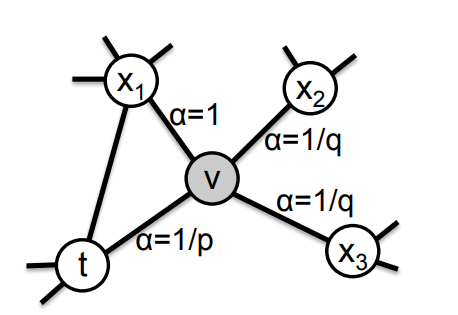
\includegraphics[width=.4\linewidth]{n2v.png}
  \caption{Random walk procedure in node2vec/ (Grover et al, 2016)}
  \label{fig:fig1}
\end{figure}
\end{itemize}

\end{itemize}
\end{frame}
%=================================================

\begin{frame}
\frametitle{IV: Latent Factor Model}
\begin{itemize}
\item Each node $i$ has an unknown latent factor $c_{i}\in R^{k}$
\vspace{10pt}
\item The probability of a node $i$  and $j$ to form a tie depends on their latent factors
 \[P(Z_{ij}=1|c_{i},c_{j})=\alpha+ c_{i}^{T} \Lambda c_{j}
    \label{3},\]  $\Lambda$ a$ K\times K$ diagonal matrix.
\vspace{10pt}
\item To run a latent factor model, the "amen" package in R-software is used,  with dimension of the multiplicative effects 1 \& 3, which measure of how likely a pair of actors are to form an edge with one another.

\end{itemize}
\end{frame}
%=================================================
\begin{frame}
\frametitle{Simulation setting}
\begin{itemize}
\item Four estimation method  considered. Each of them estimate latent variable using  dimensions 1 and 3.
\vspace{10pt}
\item{Two network studied, networks with 40 nodes and a  network with 80 nodes in two time point (T) each $T=2$ and $5$.}
\vspace{10pt}
\item{The real value of the peer influence effect is considered taking values $\beta_{2} \in \{ 0.1, 0.4, 0.7\}$ }, presenting respectively low-homofoly, mid-homofoly, high-homofoly.
\vspace{10pt}
\item{Two models involved are:}
\begin{itemize}
    \item  Influlence moddel: \[  Y_{it}=\beta_{0}+\beta_{1}Y_{i t-1}+\beta_{2} \frac{\Sigma Z_{ij t-1}Y_{j t-1}}{\Sigma Z_{ijt-1}}+ \beta_{3}X_{it-1}+\beta_{4}c_{i}+\epsilon_{it}.\] 

\item{Selection model:}
 \[ P(Z_{ij}=1|c_{i},c_{j},x_{ij},\alpha, \beta)= \Phi(\alpha+\beta |X_{i}-X_{j}|-|C_{i}-C_{j}|)
    \label{eq.4}\]
\end{itemize}
\end{itemize}
\end{frame}
%=================================================
\begin{frame}
\frametitle{Simulation results: Contagion effect }
\begin{figure}[H]
  \centering
  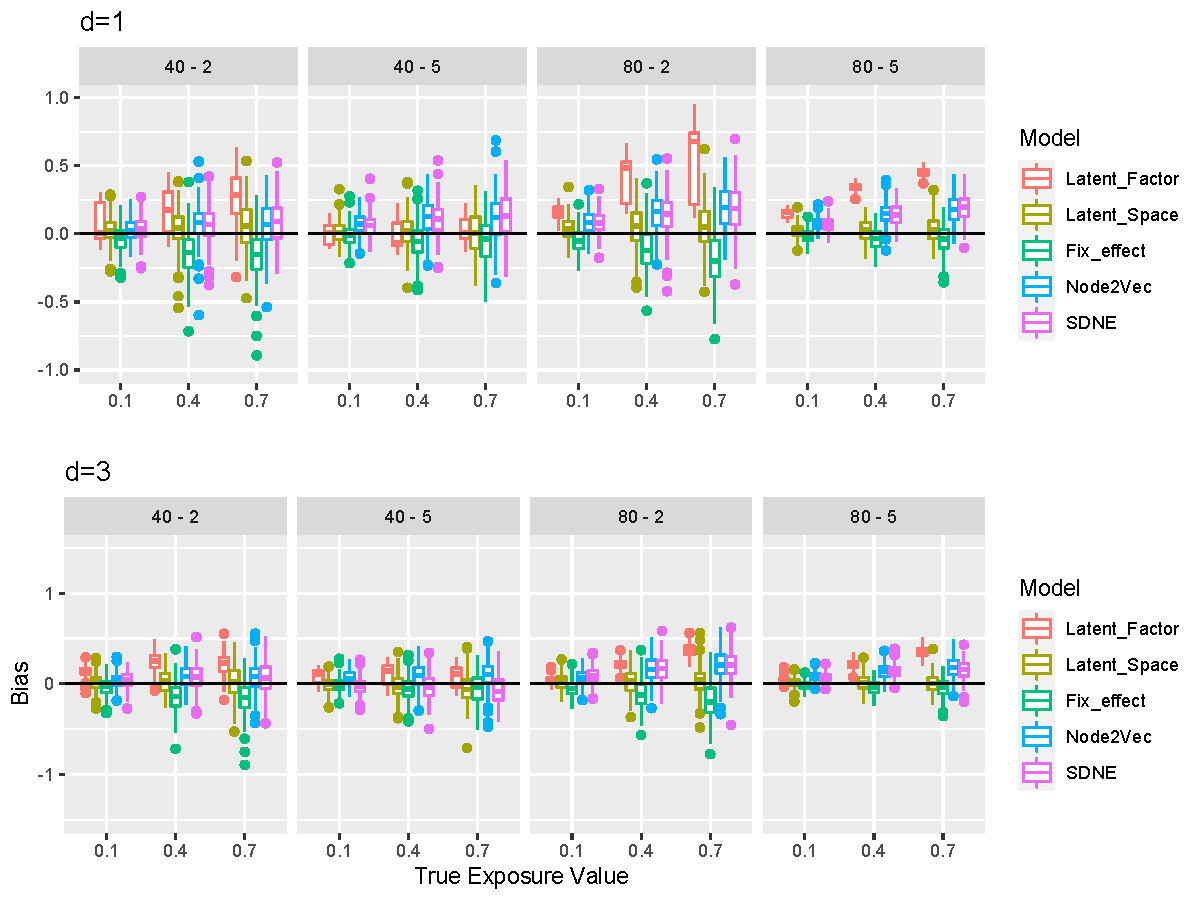
\includegraphics[width=10 cm, height=7cm ]{Rplot03after_expo.pdf}
  \caption{ Bias Distribution for Contagion Effect}
  \label{Fig:fig1}
\end{figure}

\end{frame}
%=================================================
\begin{frame}
\frametitle{ Results interpretation}
\begin{itemize}
\item  The magnitude of bias is smaller for
all estimation methods when we include more time points (T =5 bias estimate smaller than T=2).
\vspace{10pt}
\item Latent space estimates bets-perform compare to other methods in terms of estimating contagion effects, leading in smallest bias.
\vspace{10pt}
\item Overall,  Node2Vec estimates have small
bias, but performance is  better when contagion effect is small, (presence of low level of homofoly) and network size. Moving in larger network method decreases the performance. 
\vspace{10pt}
\item Latent factor estimates are more unstable,
with higher bias mostly for small dimension and small time points. Performance improved when this two factors increased.
\end{itemize}
\end{frame}
%=================================================
\begin{frame}
\frametitle{ }
\begin{itemize}

\item SDNE archived good results when network size was relatively small (almost the same bias estimation as latent space), but lost the efficiency in large networks. 
\vspace{10pt}
\item Fixed effects estimates produce the
biggest bias among all estimators.
\vspace{10pt}
\item We should point out that  the latent space and latent factor model require a large computing time, since both methods use MCMC (Marcov Chain Monte Carlo Algorithm) estimation process.
\end{itemize}
\end{frame}

%=================================================
\begin{frame}
\frametitle{Simulation Results: Latent Trait Estimation Also Help With Reducing Bias of $Y_{t-1}$ also.  }
\begin{figure}[H]
  \centering
  \includegraphics[width=10cm, height=7cm]{prior new_.pdf}
  \caption{Bias Distribution for Coefficient of Lagged Dependent Variable}
  \label{Fig:fig2}
\end{figure}
\end{frame}

%=================================================
\begin{frame}
\frametitle{ Simulation interpretation: }
\begin{itemize}
\item Latent space adjusted approach produces much smaller bias in estimating the independent variable $Y_{n-1}$ (previous behaviour) compare to other methods.
\vspace{10pt}
\item As in the contagion effect the bias  value is smaller for all estimation methods when we include more time points (compare for T=2 \& T=5).
\vspace{10pt}

\item Latent factor estimates show small bias when the true coefficient large $\beta_{1}=0.7$, but is unstable for other scenarios.
\vspace{10pt}
\item Fixed effects estimates have the larger bias and are always negatively biased.
\vspace{10pt}
\item In general Node2vec estimates  produce a small bias in contradiction to SDNE that was more efficient with contagion estimate. 
\end{itemize}
\end{frame}
%=================================================
\begin{frame}
\frametitle{Reference}
\begin{thebibliography}{10}
\begin{tiny}
\bibitem{minhas_hoff_ward_2019}
\alert{Sh. Minhas and P. D. Hoff and M. D. Ward }
\newblock  {Inferential Approaches for Network Analysis: AMEN for Latent Factor Models}
\newblock {\em  Political Analysis; 208–222, 2019. }
\bibitem{XU2018101}
\alert{R. Xu}
\newblock  {Alternative estimation methods for identifying contagion effects in dynamic social networks: A latent-space adjusted approach}
\newblock {\em Social Networks; 101-117, 2018}.

\bibitem{Friedkin1990SocialIA}
\alert{N. E. Friedkin and E. Johnsen}
\newblock {Social influence and opinions}
\newblock {\em Journal of Mathematical Sociology; 193-206, 1990. }
\bibitem{doi:10.1198/016214502388618906}
\alert{P. D. Hoff and A. E. Raftery and M. S. Handcock}
\newblock  {Latent Space Approaches to Social Network Analysis}
\newblock {\em Journal of the American Statistical Association; 1090-1098, 2002.}

\bibitem{RJ-2021-069}
\alert{R. Xu}
\newblock  {Estimating Social Influence Effects in Networks Using a Latent Space Adjusted Approach in R}
\newblock {\em The R Journal; 57-69, 2021.}
\bibitem{doi:10.1177/0049124111404820}
\alert{C. R. Shalizi and A. C. Thomas}
\newblock {Homophily and Contagion Are Generically Confounded in Observational Social Network Studies}
\newblock {\em Sociological Methods \& Research; 211-239, 2011.}

\bibitem{DBLP:journals/corr/GroverL16}
\alert{A. Grover and J. Leskovec}
\newblock  {node2vec: Scalable Feature Learning for Networks}
\newblock {\em CoRR; abs/1607.00653, 2016.}

\bibitem{10.1145/2939672.2939753}
\alert{ D.Wang and P. Cui and  W. Zhu}
\newblock  {Structural Deep Network Embedding}
\newblock {\em Association for Computing Machinery; 1225–1234, 2016.}
\newpage

\bibitem{}
\alert{ }
\newblock  {}
\newblock {\em }

\bibitem{}
\alert{ }
\newblock  {}
\newblock {\em }


\bibitem{}
\alert{ }
\newblock  {}
\newblock {\em }
\end{tiny}
\end{thebibliography}
\end{frame}
%=================================================
\end{document}
